\chapter{Components}
\label{chap:components}
% we have described many technologies in previous cgapters
% for our architecture we have chosen the following technologies
% they will be discussed in greater details

% storage/persistent streeming/real time processing scala(or additional technologies/surrounding)

\authorsection{Storage systems}{SP}

\subsection{HDFS}

\subsection{Redys}

\authorsection{Real time processing systems}{SP}

\subsection{Storm}
Batch processing cannot meet all the demands for processing Big Data.
Hadoop, the best known tool for batch processing, is helpless when it is needed to handle streaming data and obtain immediate result.
Therefore new systems, designed for real-time processing, have appeared.
One of such systems is an open source project named Storm.

Storm is a complex event-processing (CEP) system.
Complex event processing means gathering data from different sources, combining it and making conclusions from it.
For example, such system keeps track of significant changes in traffic reports or stock market feeds and immediately responds to them. 

Storm is implemented in a dialect of the Lisp language named Clojure.
Clojure is a functional language like Lisp, but it also supports multithreaded programming.
Clojure runs on the Java Virtual Machine, however applications within Storm can be written in Java, Scala, JRuby, Perl and PHP.
Moreover, one can use a Structured Query Language adapter for streaming data directly into Storm topoloy.

\mnote{Storm architecture}
The data stream consists of an unbounded set of tuples.
A tuple can contain both standard data types (integer, float, byte array) as well as user-defined types.
Every stream has its own ID.
The sources of streams called spouts. 

The next important Storm primitive is bolt.
Figure~\ref{fig:storm_architecture} shows the interaction between spouts and bolts.
The stream of tuples originates from a spout and goes through a sequence of bolts.
Every bolt performs a transformation on incoming data stream, like aggregating, filtering, or interaction with external parts such as databases.
A bolt can receive information from several spouts and stream it to multiple bolts.

\begin{figure}
  \centering
  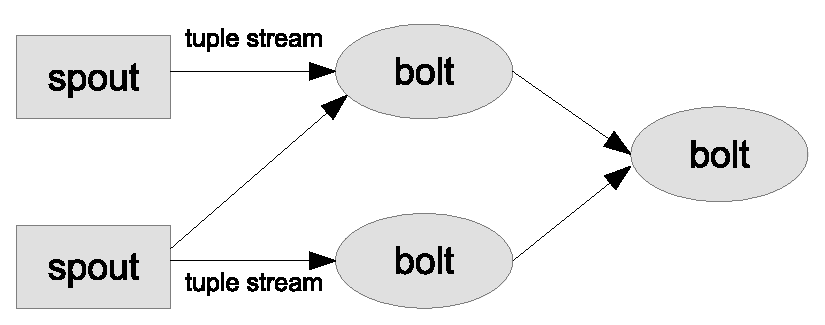
\includegraphics [width=0.9\textwidth]{images/storm_architecture}
  \caption{Storm architecture}
  \label{fig:storm_architecture}
\end{figure}

For example, MapReduce word counting example can be easily implemented with Storm.
Such system counts how many times each word occures in a given input data.
In the case of Storm one needs 
1)a spout to generate text data, 
2)one bolt to implement the Map function for word tokenisation and 
3)one bolt to implement the Reduce function for aggregation the amounts of words occurences. 

Storm allows to group the stream of tuples in different ways.
For instance, shuffle grouping randomly distributes tuples to bolts such as each bolt receives approximately the same number of tuples.
Field grouping partitions tuples according to contained fields.
Also other grouping methods exist, including the custom grouping.

The implementation charasteristics of Storm lead to high performance and fault tolerance.
It uses ZeroMQ for passing messages between the tasks.
Messages are automatically serialized and deserialized to Storm primitive types.
The usage of this message queue helps to avoid intermediate queueing, thus improving performance.
Furthermore, Storm guarantees the processing of every tuple.
In the case of a fault during message processing, a tuple is replayed from the spout.
There is also a fault detection mechanism on task level, when the failed task is quickly reasssigned to restart the processing.
Storm has supervisors to manage the processes, that leads to efficient usage of resources.

\mnote{Storm cluster}


\subsection{Scala}

\authorsection{Surrounding technologies}{SP}

\subsection{Spark}

\subsection{ZooKeeper}
Large distributed systems require a coordinator for system configuration management.
As it was mentioned in Chapter 4, Google uses a Chubby service for this purpose.
The main Chubby disadvantage is that for lock and unlock operations it is necessary to open and close the object consequently.
This feature influences the performance, increasing the time needed for making a lock.
Therefore Yahoo developes its own service named ZooKeeper that manages systems configuration and allows to efficiently lock the shared resources.

ZooKeeper namespace looks similar to a standard file system.
It consists of interconnected nodes, each of them identified by a path.
The path contains elements separated by a slash ('/').
Like in a file system, every node except the root has a parent node.
The parent node's path is a prefix for the current node path.
The ZooKeeper namespace differs from a standard file system in that its node can be a file and a directory simultaneously.

There are two types of nodes: persistent and ephemeral.
ZooKeeper stores persistent nodes on the disk, while ephemeral nodes belong to a particular session and exist only during this session.
Ephemeral nodes cannot have children nodes, they can only store data.
ZooKeeper client establishes a session with a ZooKeeper server, passing heartbeat messages.
When a client stopes to receive heartbeat messages, it reconnects to a defferent server, reestablishing the session.
If the session is canceled, all its ephemeral nodes are automatically removed.
ZooKeeper tree is presented in Figure~\ref{fig:zookeeper_tree} where the dark nodes are ephemeral.

\begin{figure}
  \centering
  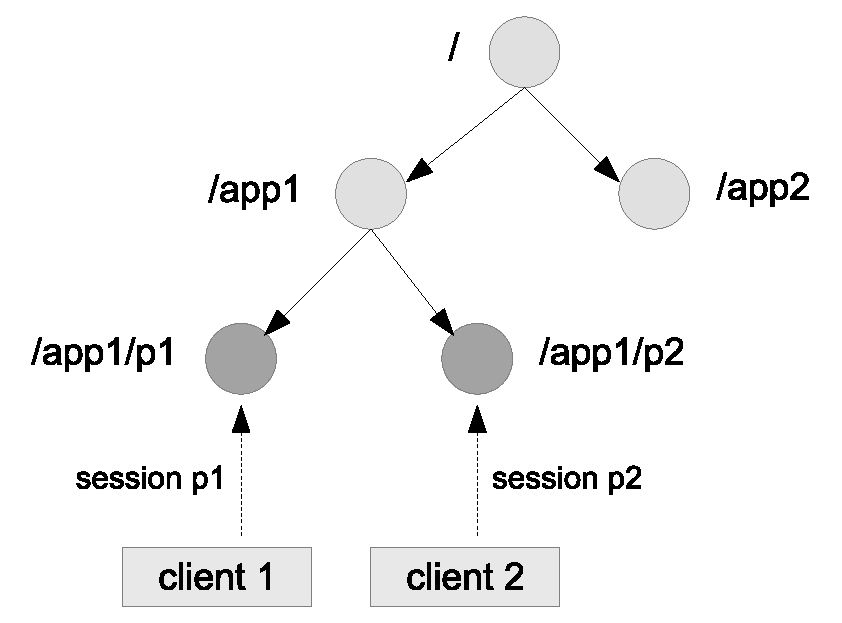
\includegraphics [width=0.9\textwidth]{images/zookeeper_tree}
  \caption{ZooKeeper tree sructure}
  \label{fig:zookeeper_tree}
\end{figure}

ZooKeeper is designed for small data warehousing, such as configuration, status and location information.
One node is usually not bigger than one kilobyte.
Therefore it stores data tree image in memory, keeping in a persistent store only transaction logs and snapshots.
In-memory storage limits the size of the database of ZooKeeper.
However, it gives advantages of low latency and high performance. 

The key feature of ZooKeeper is that it uses First In, First Out (FIFO) method for processing the messages.
It means that all commands are performed in the order they are received.
Thus, ZooKeeper maintains the total ordering.
The order is specified by a unique ZooKeeper Transaction id, that is assigned to each update.
 
ZooKeeper supports idempotent operations.
If a node should be updated, the system makes a note about the update and keeps an old and a new version of this node.
This allows client to receive the same message several times, being aware of when it can be applied.
Therefore all the write operations are performed sequentially in one thread on the master node.
However, the read request can be handled by a node's replica.
Moreover, the client also supports the total ordering of the messages.
Hence if the client sends a write request and then a read request, the write operation is performed first.
Even if usually read operation does not need a lock, ZooKeeper strictly follows the order.
It allows to implement predictable asynchronous systems that work with ZooKeeper.

The server part of ZooKeeper consists of one Leader and several Followers.
It uses two-phase commit protocol for processing updates.
During the first phase, the Leader attempts to prepare Followers to perform the steps needed to commit or abort a transaction.
This phase is also called voting phase, because the Leader receives the votes from the nodes, containing 'Yes' or 'No' reply.
In this case 'Yes' means commit and 'No' - abort.
During the second stage, the Leader performes a commit only if two of three Followers replyes 'Yes'.
Afterwards it notifies all the Followers about the result.

It can happened that one of the followers still has an outdated information when it receives the read request.
To avoid this problem, it is possible to make a force synchronisation with the master.
It is called the slow read.
Evidently, if all the clients use the slow read the system looses the advantage of scaling.
Without force synchronisation ZooKeeper system scales for reads nicely. 
However, in this case the client that reads from a replica can obtain the outdated information.

A client can watch a node.
If it sets a watch, it gets notified when the node is changed.
When the node sends this notification, it removes the watch.
In the case of connection problems between the client and the ZooKeeper server, the client receives a local notification.


\authorsection{Alternatives}{NO}